\documentclass[aspectratio=169]{beamer}

\usepackage{fontspec}
\usepackage[croatian]{babel}
\setsansfont{Latin Modern Sans}
\renewcommand{\familydefault}{\sfdefault}

\usepackage{graphicx}
\usepackage{hyperref}
\usepackage{listings}
\usepackage{xcolor}
\usepackage{tikz}

\usetheme{PaloAlto}
\usecolortheme{spruce}

\setbeamertemplate{navigation symbols}{}
\setbeamertemplate{footline}[frame number]

\title{ZORA}
\subtitle{Platforma za organizaciju rada}
\author{Tomislav Nebes}
\date{Ožujak 2025}

\begin{document}

\begin{frame}
    \titlepage
\end{frame}

\begin{frame}
    \frametitle{Sadržaj}
    \tableofcontents
\end{frame}

\section{Uvod}

\begin{frame}
    \frametitle{O aplikaciji}
    \begin{itemize}
        \item Web aplikacija za organizaciju rada
        \item Razvoj: Angular 19, .NET 9
        \item Moderno sučelje, jednostavna uporaba
    \end{itemize}
\end{frame}

\section{Arhitektura}

\begin{frame}
    \frametitle{Arhitektura sustava}
    \begin{center}
        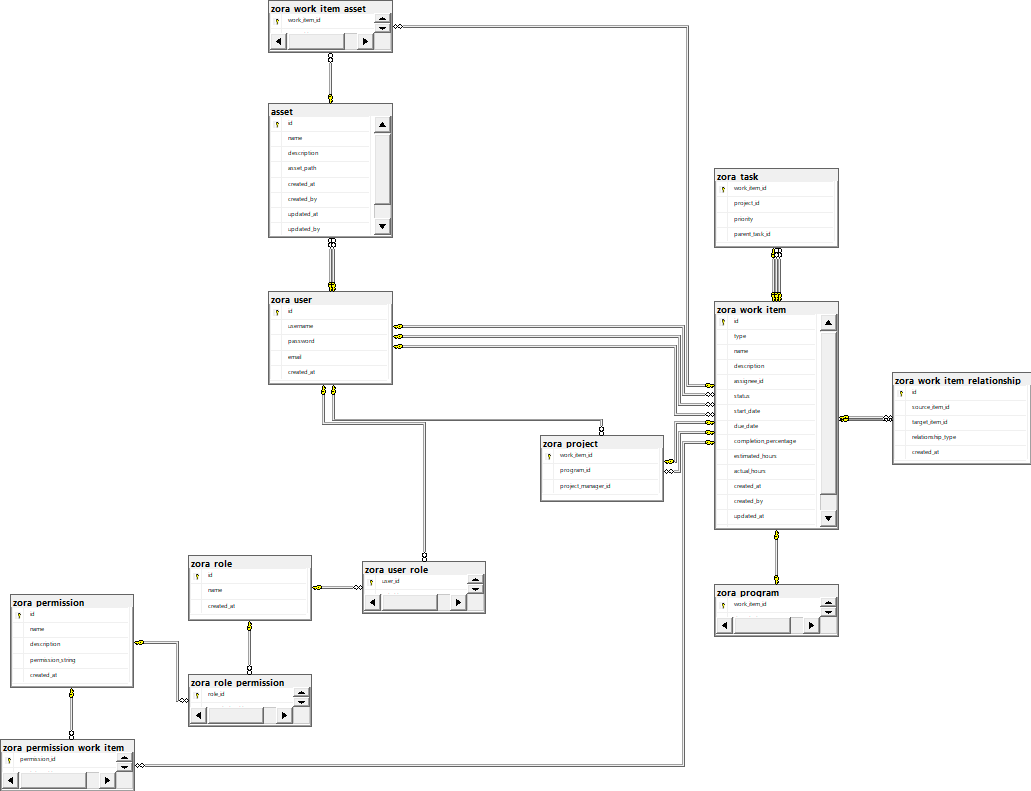
\includegraphics[height=0.75\textheight]{../zora_diagram.png}
    \end{center}
\end{frame}

\begin{frame}
    \frametitle{Deployment arhitektura i proces}
    \begin{itemize}
        \item VPS (Ubuntu Server 22.04 LTS)
        \item Nginx reverse proxy, SSL (Let's Encrypt)
        \item Systemd backend service
        \item CI/CD putem Jenkins (webhook)
        \item Monitoring (journalctl)
    \end{itemize}
\end{frame}

\section{Backend}

\begin{frame}
    \frametitle{Backend tehnologije}
    \begin{itemize}
        \item .NET 9 Web API, Entity Framework Core
        \item SQL Server, JWT, Swagger
        \item AutoMapper, Dapper, FluentResults
        \item Serilog, Bcrypt.Net, CryptoHelper
    \end{itemize}
\end{frame}

\begin{frame}
    \frametitle{Backend struktura}
    \begin{columns}
        \begin{column}{0.45\textwidth}
            \begin{itemize}
                \item Clean Architecture
                \begin{itemize}
                    \item Controllers
                    \item Services
                    \item Repositories
                    \item Models, DTOs
                \end{itemize}
                \item Dependency Injection
                \item Middleware
            \end{itemize}
        \end{column}
        \begin{column}{0.6\textwidth}
            \textbf{Struktura direktorija:}
            \begin{itemize}
                \item \texttt{app/src/}
                \begin{itemize}
                    \item \texttt{API/}
                    \begin{itemize}
                        \item Controllers
                        \item Mapping
                        \item Interfaces
                        \item Middleware
                    \end{itemize}
                    \item \texttt{Core/}
                    \begin{itemize}
                        \item Domain
                        \item DTOs
                        \item Interfaces
                        \item Enums
                    \end{itemize}
                    \item \texttt{Infrastructure/}
                    \begin{itemize}
                        \item Controllers
                        \item Services
                        \item Repositories
                        \item Data
                    \end{itemize}
                \end{itemize}
            \end{itemize}
        \end{column}
    \end{columns}
\end{frame}

\section{Frontend}

\begin{frame}
    \frametitle{Frontend tehnologije}
    \begin{itemize}
        \item Angular 19, Angular Material
        \item RxJS, NgRx (State management)
        \item Jest (Testiranje)
    \end{itemize}
\end{frame}

\begin{frame}
    \frametitle{Frontend struktura}
    \begin{itemize}
        \item Feature-based moduli
        \item Lazy loading, Interceptors, Guards
        \item Core, Shared, Auth moduli
    \end{itemize}
\end{frame}

\section{Demo}

\begin{frame}
    \frametitle{Demo koraci}
    \begin{enumerate}
        \item prijava u sustav s administratorskim pristupom
        \item Swagger i ERA dijagram
        \item pregledavanje profila
        \item stvaranje zadatka s resursom
        \item pregled kontrolne ploče i pregled resursa iz kontrolne ploče
        \item stvaranje ovlasti nad zadatkom
        \item stvaranje uloge sa ovlašću
        \item stvaranje korisnika s ulogom
        \item postavljanje novog korisnika kao izvršavatelja zadatka
        \item prijava s novim korisnikom
        \item pregled zadatka i resursa
        \item završetak zadatka
    \end{enumerate}
\end{frame}

\section{Zaključak}

\begin{frame}
    \frametitle{Zaključak}
    \begin{itemize}
        \item Implementirana web aplikacija
        \item Skalabilno i održivo rješenje
        \item Napredno upravljanje zadacima
        \item Integrirano praćenje i izvještavanje
    \end{itemize}
\end{frame}

\begin{frame}
    \frametitle{Pitanja?}
    \begin{center}
        {\Huge Hvala.}
    \end{center}
\end{frame}

\end{document}